\begin{figure}[hbtp]
  \centering
  \subfigure{
    \label{fig:about-hashtable--all}
    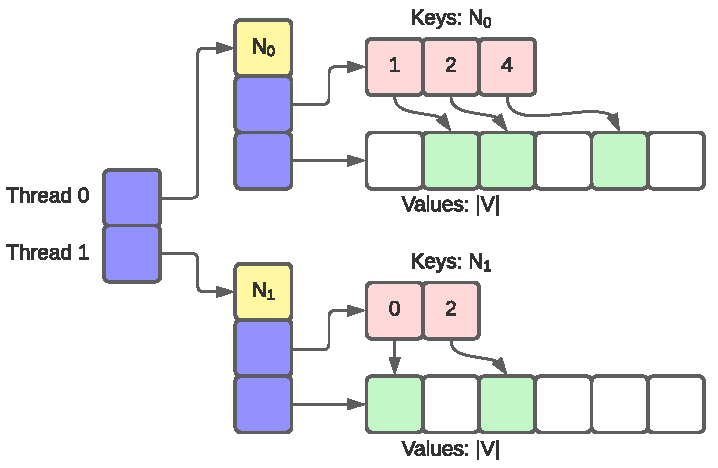
\includegraphics[width=0.88\linewidth]{out/about-hashtable.pdf}
  } \\[-2ex]
  \caption{Illustration of collision-free per-thread hashtables that are well separated in their memory addresses, for two threads. Each hashtable consists of a keys vector, values vector (of size $|V|$), and a key count ($N_0$/$N_1$). The value associated with each key is stored/accumulated in the index pointed by the key. As the key count of each hashtable is updated independently, we allocate it separately on the heap to avoid false cache sharing. These are used in the scoring phase of our implementation to keep track of common neighbors between a pair of vertices, i.e., between the given vertex $i$, and its second degree neighbors.}
  \label{fig:about-hashtable}
\end{figure}
